\documentclass[10.5pt]{article}

% Packages:
\usepackage[utf8]{inputenc}
\usepackage[english]{babel}
\usepackage{float}
\usepackage{graphicx}
\usepackage{amssymb}
\usepackage{bm}
\usepackage{mathtools}          %loads amsmath as well
\usepackage{indentfirst}
\usepackage{tikz}
%\usepackage{pgfplots}
%\usepackage{titling}
%\usepackage{biblatex}
\DeclareGraphicsRule{.tif}{png}{.png}{`convert #1 `dirname #1`/`basename #1 .tif`.png}

% Move title up:
%\setlength{\droptitle}{-10em}

\begin{document}

% Title information:
\title{Average-Interpolating Wavelet Scheme}
\author{Brandon Gusto}
\maketitle

% first section on interpolating (predict) stage
\section*{Multiresolution Analysis Procedure}
We are interested in obtaining the difference between approximation spaces at varying levels of resolution. We 
are given cell-averaged values as input data to our wavelet transform. This data is fed to the scheme at some arbitrary maximum
resolution level $J$, and the wavelet transform produces details coefficients at each lower level until the coarsest level,
$j=0$, is reached. The coefficients in this case are interchangeable with the cell-averages and are denoted by $c^{j}_{k}$,
where the level of resolution is denoted by $j$, and the spatial index is denoted by $k$. We consider an interpolating
polynomial $p(x)$ such that 
\begin{align}
    c^{j}_{k-1} &= \int_{x^{j}_{k-1}}^{x^{j}_{k}} p(x) dx \\
    c^{j}_{k} &= \int_{x^{j}_{k}}^{x^{j}_{k+1}} p(x) dx \\
    c^{j}_{k+1} &= \int_{x^{j}_{k+1}}^{x^{j}_{k+2}} p(x) dx.
\end{align}
The polynomial $p(x)$ should then predict the finer cell-averages of cell $c^{j}_{k}$ as
\begin{align}
    \hat{c}^{j+1}_{2k} &= 2 \int_{x^{j}_{k}}^{x^{j}_{k+1/2}} p(x) dx \\
    \hat{c}^{j+1}_{2k+1} &= 2 \int_{x^{j}_{k+1/2}}^{x^{j}_{k+1}} p(x) dx
\end{align}
At present, it may not be clear how to implement such a scheme on a computer. However this interpolation procedure
can be cast in a more suitable form by introducing another polynomial, the integral of $p(x)$:
\begin{equation}
	P(x) = \int_{0}^{x} p(y) dy.
\end{equation}
Now the problem is to interpolate the following data
\begin{align}
    0 &= P(x^{j}_{k-1}) \\
    c^{j}_{k-1} &= P(x^{j}_{k}) \\
    c^{j}_{k-1} + c^{j}_{k} &= P(x^{j}_{k+1}) \\
    c^{j}_{k-1} + c^{j}_{k} + c^{j}_{k+1} &= P(x^{j}_{k+2}).
\end{align}
This can easily be done using Lagrange polynomials. Then the predictions are given in terms of $P(x)$ by
\begin{align}
	\hat{c}^{j+1}_{2k} &= 2 \left( P(x^{j}_{k+1/2}) - P(x^{j}_{k}) \right) \\
	\hat{c}^{j+1}_{2k+1} &= 2 \left( P(x^{j}_{k+1}) - P(x^{j}_{k+1/2}) \right).
\end{align}
This interpolating polynomial is cast in the Lagrange form,
\begin{equation}
P(x) = \sum_{i=0}^{n} y_{i} l_{i}(x),
\end{equation}
where $y_{i}$ are the functional data, and $l_{i}(x)$ are the Lagrange polynomials. For $n=3$ these
are given by
\begin{align}
    l_{0}(x) &= \frac{x-x_1}{x_0-x_1} \frac{x-x_2}{x_0-x_2} \frac{x-x_3}{x_0-x_3} \\
    l_{1}(x) &= \frac{x-x_0}{x_1-x_0} \frac{x-x_2}{x_1-x_2} \frac{x-x_3}{x_1-x_3} \\
    l_{2}(x) &= \frac{x-x_0}{x_1-x_0} \frac{x-x_1}{x_2-x_1} \frac{x-x_3}{x_2-x_3} \\
    l_{3}(x) &= \frac{x-x_0}{x_3-x_0} \frac{x-x_1}{x_3-x_1} \frac{x-x_2}{x_3-x_2},
\end{align}
and the final interpolating polynomial is
\begin{equation}
	P(x) = (0) l_{0}(x) + ( c^{j}_{k-1} ) l_{1}(x) + ( c^{j}_{k-1} + c^{j}_{k} ) l_{2}(x)
		+ ( c^{j}_{k-1} + c^{j}_{k} + c^{j}_{k+1} ) l_{3}(x).
\end{equation}
Several evaluations are necessary in order to obtain the predictions. Using intervals of equal length, these values are
\begin{align}
	P(x^{j}_{k}) &= c^{j}_{k-1} \\
	P(x^{j}_{k+1/2}) &= \frac{17}{16} c^{j}_{k-1} + \frac{1}{2} c^{j}_{k} - \frac{1}{16} c^{j}_{k+1} \\
	P(x^{j}_{k+1}) &= c^{j}_{k-1} + c^{j}_{k}.
\end{align}
Then the predictions of the cell-averages at the higher level of resolution are finally given by
\begin{align}
	\hat{c}^{j+1}_{2k} = c^{j}_{k} + \frac{1}{8} \left( c^{j}_{k-1} - c^{j}_{k+1} \right) \\
	\hat{c}^{j+1}_{2k+1} = c^{j}_{k} - \frac{1}{8} \left( c^{j}_{k-1} - c^{j}_{k+1} \right).
\end{align}
This procedure could easily be extended to non-uniformly spaced intervals, giving different weights. The detail,
or wavelet coefficient on level $j$ is then given by the difference between known value and prediction,
\begin{equation}
	d^{j}_{k} = c^{j+1}_{2k+1} - \hat{c}^{j+1}_{2k+1}.
\end{equation}
Note that only the odd indices are counted because in the multiresolution scheme the data is initially split into even
and odd signals. All data at level $j$ are just considered to be a copy of the even-index data at level $j+1$, whereas
the odd-indexed data at level $j+1$ is what is predicted by even-indexed data at level $j+1$.

% cell average drawing
\begin{figure}
    \centering
    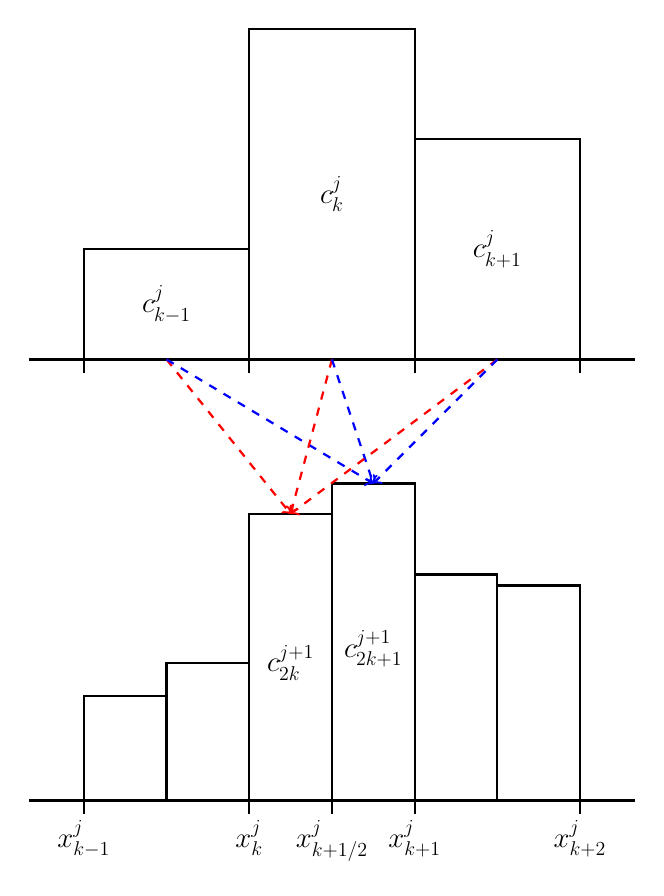
\begin{tikzpicture}[thick,scale=0.7, every node/.style={scale=0.6}]
        \draw (0,0) -- (0,2)-- (3,2);
        \draw (3,0) -- (3,6) -- (6,6) -- (6,0);
        \draw (6,0) -- (6,4) -- (9,4) -- (9,0);
        \draw (-1,0) -- (10,0);
        \node at (1.5,1) {\LARGE $c^{j}_{k-1}$};
        \node at (4.5,3) {\LARGE $c^{j}_{k}$};
        \node at (7.5,2) {\LARGE $c^{j}_{k+1}$};
        \draw (0,0) -- (0,-0.25);
        \draw (3,0) -- (3,-0.25);
        \draw (6,0) -- (6,-0.25);
        \draw (9,0) -- (9,-0.25);

        % -8 is y-axis baseline for this one
        \draw (0,-8) -- (0,-6.1) -- (1.5,-6.1) -- (1.5,-8);
        \draw (1.5,-8) -- (1.5,-5.5) -- (3,-5.5) -- (3,-8);
        \draw (3,-8) -- (3,-2.8) -- (4.5,-2.8) -- (4.5,-8);
        \draw (4.5,-8) -- (4.5,-2.25) -- (6,-2.25) -- (6,-8);
        \draw (6,-8) -- (6,-3.9) -- (7.5,-3.9) -- (7.5,-8);
        \draw (7.5,-8) -- (7.5,-4.1) -- (9,-4.1) -- (9,-8);
        \draw (-1,-8) -- (10,-8);
        \node at (3.75,-5.5) {\LARGE $c^{j+1}_{2k}$};
        \node at (5.25,-5.25) {\LARGE $c^{j+1}_{2k+1}$};
	\draw (0,-8) -- (0,-8.25);
        \draw (3,-8) -- (3,-8.25);
        \draw (4.5,-8) -- (4.5,-8.25);
        \draw (6,-8) -- (6,-8.25);
	\draw (9,-8) -- (9,-8.25);

        % arrows
        \draw[red,dashed,->] (1.5,0) -- (3.75,-2.8);
        \draw[blue,dashed,->] (1.5,0) -- (5.25,-2.25);
        \draw[red,dashed,->] (4.5,0) -- (3.75,-2.8);
        \draw[blue,dashed,->] (4.5,0) -- (5.25,-2.25);
        \draw[red,dashed,->] (7.5,0) -- (3.75,-2.8);
        \draw[blue,dashed,->] (7.5,0) -- (5.25,-2.25);

        % tick text
        \node[below] at (0,-8.25) {\LARGE $x^{j}_{k-1}$};
        \node[below] at (3,-8.25) {\LARGE $x^{j}_{k}$};
        \node[below] at (4.5,-8.25) {\LARGE $x^{j}_{k+1/2}$};
        \node[below] at (6,-8.25) {\LARGE $x^{j}_{k+1}$};
        \node[below] at (9,-8.25) {\LARGE $x^{j}_{k+2}$};

    \end{tikzpicture}
    \caption{Quadratic prediction operator from coarse-scale $j$ to fine-scale $j+1$, given cell-averaged data $\mathbf{c}^{j}$. 
		Red and Blue arrows indicate interpolation dependency for each of the new cells, $c^{j}_{2k}$ and $c^{j}_{2k+1}$,
		respectively.}

\end{figure}

\end{document}
